\begin{equation}
    \begin{gathered}
        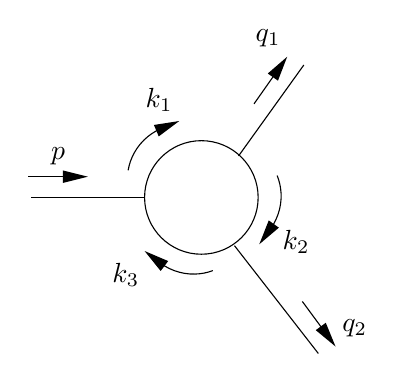
\begin{tikzpicture}[x=0.75pt,y=0.75pt,yscale=-1,xscale=1]
            %uncomment if require: \path (0,300); %set diagram left start at 0, and has height of 300
            
            %Shape: Circle [id:dp004805450328669414] 
            \draw   (204,151.35) .. controls (204,136.25) and (216.25,124) .. (231.35,124) .. controls (246.46,124) and (258.71,136.25) .. (258.71,151.35) .. controls (258.71,166.46) and (246.46,178.71) .. (231.35,178.71) .. controls (216.25,178.71) and (204,166.46) .. (204,151.35) -- cycle ;
            %Straight Lines [id:da15453068055760366] 
            \draw    (149.29,151.35) -- (204,151.35) ;
            %Straight Lines [id:da6670631824254709] 
            \draw    (249.29,131.35) -- (280.71,87.56) ;
            %Straight Lines [id:da8512297070729149] 
            \draw    (247.29,174.56) -- (287.71,226.53) ;
            %Straight Lines [id:da12241887785336236] 
            \draw    (147.94,141.35) -- (174.65,141.35) ;
            \draw [shift={(176.65,141.35)}, rotate = 180] [fill={rgb, 255:red, 0; green, 0; blue, 0 }  ][line width=0.08]  [draw opacity=0] (12,-3) -- (0,0) -- (12,3) -- cycle    ;
            %Straight Lines [id:da04852909152903351] 
            \draw    (256.71,106.28) -- (271.55,85.19) ;
            \draw [shift={(272.71,83.56)}, rotate = 485.15] [fill={rgb, 255:red, 0; green, 0; blue, 0 }  ][line width=0.08]  [draw opacity=0] (12,-3) -- (0,0) -- (12,3) -- cycle    ;
            %Straight Lines [id:da8349858256899048] 
            \draw    (280,201.46) -- (294.81,221.57) ;
            \draw [shift={(296,223.18)}, rotate = 233.63] [fill={rgb, 255:red, 0; green, 0; blue, 0 }  ][line width=0.08]  [draw opacity=0] (12,-3) -- (0,0) -- (12,3) -- cycle    ;
            %Shape: Arc [id:dp6371346371514501] 
            \draw  [draw opacity=0] (196.08,138.27) .. controls (196.56,135.45) and (197.49,132.69) .. (198.91,130.07) .. controls (202.29,123.8) and (207.87,119.41) .. (214.36,117.2) -- (226.47,144.96) -- cycle ; \draw   (196.08,138.27) .. controls (196.56,135.45) and (197.49,132.69) .. (198.91,130.07) .. controls (202.29,123.8) and (207.87,119.41) .. (214.36,117.2) ;
            %Straight Lines [id:da025947757177437136] 
            \draw    (214.36,117.2) -- (218.86,115.3) ;
            \draw [shift={(220.71,114.53)}, rotate = 517.11] [fill={rgb, 255:red, 0; green, 0; blue, 0 }  ][line width=0.08]  [draw opacity=0] (12,-3) -- (0,0) -- (12,3) -- cycle    ;
            
            %Shape: Arc [id:dp055990585045730734] 
            \draw  [draw opacity=0] (267.88,140.82) .. controls (268.94,143.47) and (269.59,146.31) .. (269.75,149.29) .. controls (270.13,156.4) and (267.66,163.06) .. (263.27,168.33) -- (238.47,150.96) -- cycle ; \draw   (267.88,140.82) .. controls (268.94,143.47) and (269.59,146.31) .. (269.75,149.29) .. controls (270.13,156.4) and (267.66,163.06) .. (263.27,168.33) ;
            %Straight Lines [id:da03941082214307445] 
            \draw    (263.27,168.33) -- (260.42,172.29) ;
            \draw [shift={(259.26,173.92)}, rotate = 305.67] [fill={rgb, 255:red, 0; green, 0; blue, 0 }  ][line width=0.08]  [draw opacity=0] (12,-3) -- (0,0) -- (12,3) -- cycle    ;
            
            %Shape: Arc [id:dp9228997543552979] 
            \draw  [draw opacity=0] (236.87,186.62) .. controls (234.19,187.61) and (231.33,188.19) .. (228.35,188.27) .. controls (221.23,188.47) and (214.64,185.84) .. (209.48,181.32) -- (227.47,156.96) -- cycle ; \draw   (236.87,186.62) .. controls (234.19,187.61) and (231.33,188.19) .. (228.35,188.27) .. controls (221.23,188.47) and (214.64,185.84) .. (209.48,181.32) ;
            %Straight Lines [id:da046155827300820684] 
            \draw    (209.48,181.32) -- (205.59,178.37) ;
            \draw [shift={(203.99,177.16)}, rotate = 397.11] [fill={rgb, 255:red, 0; green, 0; blue, 0 }  ][line width=0.08]  [draw opacity=0] (12,-3) -- (0,0) -- (12,3) -- cycle    ;
            
            
            % Text Node
            \draw (162.29,136.95) node [anchor=south] [inner sep=0.75pt]    {$p$};
            % Text Node
            \draw (270.71,80.16) node [anchor=south east] [inner sep=0.75pt]    {$q_{1}$};
            % Text Node
            \draw (298,219.78) node [anchor=south west] [inner sep=0.75pt]    {$q_{2}$};
            % Text Node
            \draw (218.71,111.13) node [anchor=south east] [inner sep=0.75pt]    {$k_{1}$};
            % Text Node
            \draw (269.27,165.73) node [anchor=north west][inner sep=0.75pt]    {$k_{2}$};
            % Text Node
            \draw (187.27,181.73) node [anchor=north west][inner sep=0.75pt]    {$k_{3}$};
            \end{tikzpicture}
    \end{gathered} = (\ii g)^3 \frac{\ii}{k_1^2 - m^2 + \ii 0^+} \frac{\ii}{k_2^2 - m^2 + \ii 0^+} \frac{\ii}{k_3^2 - m^2 + \ii 0^+},
    \label{eq:phi-phiphi-no-integral-one-loop}
\end{equation}